\chapter{Error-State Dynamics and Covariance Propagation}
\label{ch:errordyn}
\chaptermark{Error-State Dynamics} % short running header

\begin{objectives}
\begin{itemize}
  \item Set up the 15-dimensional IMU error state with the frozen index layout.
  \item Derive linearized error dynamics with the four-step recipe, including the attitude error under a
        perturbation convention.
  \item Discretize into $\Phi$ and $Q_d$ and propagate the covariance of the IMU state and its clones.
  \item Predict analytically how fast each noise source inflates the position uncertainty.
  \item Validate the propagation by finite differences and by Monte Carlo simulation.
\end{itemize}
\end{objectives}

% ------------------------------------------------------------------------------
\section{True and nominal systems}

The true state evolves under the IMU model \eqref{eq:imu-model} solved for the physical quantities. With
$\omega = \omega_m - b_g - n_g$ and $a = a_m - b_a - n_a$ the true body rate and specific force,
\begin{equation}
  \dot p = v, \qquad \dot v = R\,(a_m - b_a - n_a) + g_w, \qquad \dot R = R\,\sx{\omega_m - b_g - n_g},
  \qquad \dot b_a = n_{b_a}, \qquad \dot b_g = n_{b_g},
  \label{eq:true-ct}
\end{equation}
where $R = R_{wb}$. The nominal state follows \eqref{eq:nominal-ct}, which is \eqref{eq:true-ct} with the biases replaced
by their estimates and the noise set to zero. The error state measures their difference.

\begin{convention}[error-state layout, AGENTS.md C3]
\begin{center}\small
\begin{tabular}{@{}c c l@{}}
\toprule
Indices & Block & Meaning \\
\midrule
0--2 & $\delta p$ & position error, world frame \\
3--5 & $\delta v$ & velocity error, world frame \\
6--8 & $\delta\theta$ & attitude error, \textbf{body frame (local)}: $R = \hat R\Exp(\delta\theta)$ \\
9--11 & $\delta b_a$ & accelerometer bias error \\
12--14 & $\delta b_g$ & gyroscope bias error \\
$15+6i$ \dots $+2$ & $\delta p_i$ & clone $i$ position error \\
$18+6i$ \dots $+2$ & $\delta\theta_i$ & clone $i$ attitude error (local) \\
\bottomrule
\end{tabular}
\end{center}
Noise ordering: $w = [n_a, n_g, n_{b_a}, n_{b_g}] \in \R^{12}$.
\end{convention}

Index constants belong in one place in the code (\code{constexpr} offsets in \code{types.hpp}), and every block
access goes through them. Hard-coded literals such as \code{P.block<3,3>(6,6)} scattered through the code are how
layout bugs are born.

% ------------------------------------------------------------------------------
\section{Deriving the error dynamics}
\label{sec:deriving-Fc}

The goal is the linear system
\begin{equation}
  \dot{\delta x}_I = F_c\,\delta x_I + G_c\,w, \qquad F_c \in \R^{15\times15},\quad G_c \in \R^{15\times12},
\end{equation}
obtained with the recipe of \cref{sec:error-dyn-recipe}. Two of the five blocks are immediate.

\paragraph{Position.} Substituting $p = \hat p + \delta p$ and $v = \hat v + \delta v$ into $\dot p = v$ and subtracting
$\dot{\hat p} = \hat v$ gives $\dot{\delta p} = \delta v$ exactly. No linearization is needed.

\paragraph{Biases.} $\dot b_a = n_{b_a}$ and $\dot{\hat b}_a = 0$ give $\dot{\delta b}_a = n_{b_a}$, and likewise
$\dot{\delta b}_g = n_{b_g}$.

The velocity and attitude blocks involve the rotation and require the Lie tools of \cref{ch:lie}. One lemma
handles the time derivative of the perturbation itself.

\begin{lemma}[Time derivative of a perturbation]
\label{lem:dexp}
For a differentiable $\delta\theta(t)$,
$\frac{\dd}{\dd t}\Exp(\delta\theta) = \Exp(\delta\theta)\sx{\Jr(\delta\theta)\,\dot{\delta\theta}} = \sx{\Jl(\delta\theta)\,\dot{\delta\theta}}\Exp(\delta\theta)$.
To first order in $\delta\theta$, both reduce to $\sx{\dot{\delta\theta}}$ multiplying $\Exp(\delta\theta)$ on the corresponding side.
\end{lemma}
\begin{proof}
Apply the definition \eqref{eq:jr-def} of $\Jr$ and $\Jl$ with $\delta = \dot{\delta\theta}\,\dd t$.
\end{proof}

\subsection{Worked example: attitude error under the global perturbation}

To demonstrate the method without solving the project's exercise, we first derive the attitude error
dynamics for the \emph{global} perturbation $R = \Exp(\delta\theta_g)\hat R$. This is \textbf{not} the project's
convention; it is here for contrast.

\begin{example}[Global attitude error dynamics]
\label{ex:global-attitude}
Differentiate both sides of $R = \Exp(\delta\theta_g)\hat R$ using \cref{lem:dexp} to first order and the kinematics
$\dot R = R\sx{\omega}$, $\dot{\hat R} = \hat R\sx{\hat\omega}$:
\begin{equation*}
  \underbrace{\Exp(\delta\theta_g)\hat R\sx{\omega}}_{\dot R}
  \approx \sx{\dot{\delta\theta}_g}\Exp(\delta\theta_g)\hat R + \Exp(\delta\theta_g)\hat R\sx{\hat\omega}.
\end{equation*}
Move the last term to the left and use $\omega - \hat\omega = -\delta b_g - n_g$:
\begin{equation*}
  \sx{\dot{\delta\theta}_g}\Exp(\delta\theta_g)\hat R \approx \Exp(\delta\theta_g)\hat R\sx{-\delta b_g - n_g}.
\end{equation*}
Multiply on the right by $(\Exp(\delta\theta_g)\hat R)\T$ and apply \eqref{eq:skew-rot} with the rotation $\Exp(\delta\theta_g)\hat R$:
\begin{equation*}
  \sx{\dot{\delta\theta}_g} \approx \sx{\Exp(\delta\theta_g)\hat R(-\delta b_g - n_g)} \approx \sx{-\hat R\,\delta b_g - \hat R\, n_g},
\end{equation*}
where the last step drops the product of $\delta\theta_g$ with $\delta b_g$ and $n_g$, both small. Hence
\begin{equation}
  \dot{\delta\theta}_g = -\hat R\,\delta b_g - \hat R\,n_g .
\end{equation}
The global attitude error does not depend on itself at all: the world-frame error is constant unless driven by
gyro errors, which are rotated into the world by $\hat R$.
\end{example}

\subsection{Your turn: the local (right) perturbation}

\begin{derivex}{attitude and velocity rows of $F_c$ and $G_c$}{sol:Fc}
Derive $\dot{\delta\theta}$ and $\dot{\delta v}$ under the project's local perturbation $R = \hat R\Exp(\delta\theta)$.
\begin{enumerate}
  \item \textbf{Attitude.} Differentiate $R = \hat R\Exp(\delta\theta)$ with \cref{lem:dexp} (right form). Cancel the nominal
        term, then use $\Exp(-\delta\theta)\sx{\hat\omega}\Exp(\delta\theta) = \sx{\Exp(-\delta\theta)\hat\omega}$ and
        $\Exp(-\delta\theta)\hat\omega \approx \hat\omega - \delta\theta\times\hat\omega$. You should find a term proportional to $\delta\theta$ that the global
        version lacks. Explain it physically: what happens to a body-frame error when the body rotates?
  \item \textbf{Velocity.} Substitute $R = \hat R\Exp(\delta\theta) \approx \hat R(I + \sx{\delta\theta})$ and
        $a_m - b_a - n_a = \hat a - \delta b_a - n_a$ into $\dot v = R(a_m - b_a - n_a) + g_w$, subtract
        $\dot{\hat v} = \hat R\hat a + g_w$, drop second-order products, and use \eqref{eq:skew-anticomm} to move $\delta\theta$ to the
        right.
  \item \textbf{Assemble} $F_c$ and $G_c$ in the frozen order of AGENTS.md C3. Before filling any block, predict
        from the cascade structure of the kinematics which blocks must be zero.
\end{enumerate}
\textbf{Check:} build $\Phi \approx I + F_c\Dt$ and compare each column with
$\big(f(\hat x\bplus\epsilon e_i)\bminus f(\hat x)\big)/\epsilon$ for one step $f$ of your nominal integrator, at a state with
non-identity attitude, non-zero rates, specific force and biases (Milestone 5). Agreement must be at the level
of the $O(\Dt^2)$ terms neglected by $I + F_c\Dt$. Then record the result in \code{DOCS/derivations.md}.
\end{derivex}

Physically, the velocity row you will find encodes the most important coupling in inertial navigation: an
attitude error tilts the computed specific force, so a fraction of the large vector $\hat a$ (dominated by the
reaction to gravity, $9.81~\mathrm{m/s^2}$) leaks into the velocity error. That single term is behind the
$t^3$ law of \cref{ch:intro}.

% ------------------------------------------------------------------------------
\section{Discretization}

Over one IMU step the error dynamics are discretized as in \cref{sec:discretization} (AGENTS.md F2):
\begin{equation}
  \Phi \approx I_{15} + F_c\Dt, \qquad
  Q_c = \diag\big(\sigma_a^2 I_3,\ \sigma_g^2 I_3,\ \sigma_{b_a}^2 I_3,\ \sigma_{b_g}^2 I_3\big), \qquad
  Q_d \approx G_c Q_c G_c\T\Dt ,
  \label{eq:imu-discretization}
\end{equation}
with $F_c$ and $G_c$ evaluated at the nominal state and the bias-corrected IMU inputs at the beginning of the
step (or at the midpoint, consistently with the chosen integration scheme). The densities are the
continuous-time values of \cref{tab:euroc-imu}; the $\Dt$ in $Q_d$ converts them into variances
accumulated during the step.

\begin{remark}[higher-order options]
$F_c$ is block upper-triangular with a large nilpotent part, so $\exp(F_c\Dt)$ has a closed form. In particular the
attitude block of the exact $\Phi$ is a rotation matrix, while the first-order block is not exactly orthogonal. At
200~Hz and 1~rad/s the difference per step is about $(\|\hat\omega\|\Dt)^2/2 \approx 10^{-5}$, below the noise.
Adopting a higher-order $\Phi$ is allowed if it is logged (AGENTS.md F2). Van Loan's method
(\cref{prop:vanloan}) gives exact reference values for testing whichever form is used.
\ifsolutions The closed-form blocks are listed with the solutions in \cref{sol:Phi}.\fi
\end{remark}

\paragraph{The continuous-time view.} The discrete recursion is a numerical integration of a differential equation for the covariance.
For the linear stochastic system $\dot{\delta x} = F_c\,\delta x + G_c\,w$, the covariance obeys the Lyapunov differential equation of
\cref{prop:lyapunov},
\begin{equation}
  \dot P = F_cP + PF_c\T + G_cQ_cG_c\T .
  \label{eq:imu-lyapunov}
\end{equation}
Substituting $\Phi = I + F_c\Dt$ and $Q_d = G_cQ_cG_c\T\Dt$ into one step gives
$\Phi P\Phi\T + Q_d = P + \big(F_cP + PF_c\T + G_cQ_cG_c\T\big)\Dt + F_cPF_c\T\Dt^2$: the filter's propagation is Euler's method applied to
\eqref{eq:imu-lyapunov}, with a local error of $O(\Dt^2)$. Each term has a meaning. $G_cQ_cG_c\T$ injects uncertainty where the noise enters (velocity,
attitude and the biases), and $F_cP + PF_c\T$ transports it along the couplings of $F_c$: from biases into attitude and velocity, from attitude into
velocity, from velocity into position. The growth laws of \cref{prop:growth-laws} below are exact solutions of \eqref{eq:imu-lyapunov} for a level,
stationary IMU, and they are the reference against which the discrete propagation is tested in Milestone 5.

% ------------------------------------------------------------------------------
\section{Propagating the full covariance}

With $N$ clones the state has dimension $n = 15 + 6N$, and the covariance is partitioned as
\begin{equation}
  P = \begin{bmatrix} P_{II} & P_{IC} \\ P_{CI} & P_{CC} \end{bmatrix},
  \qquad P_{II}\in\R^{15\times15},\ P_{IC}\in\R^{15\times6N},\ P_{CC}\in\R^{6N\times6N}.
\end{equation}
Clones are frozen copies of past poses, so their error dynamics are zero: $\dot{\delta x}_C = 0$. The full
transition matrix is $\blkdiag(\Phi, I_{6N})$, and the full process noise is $\blkdiag(Q_d, 0)$. Multiplying out:

\begin{convention}[covariance propagation, AGENTS.md F2]
\begin{equation}
  P_{II} \gets \Phi P_{II}\Phi\T + Q_d, \qquad P_{IC} \gets \Phi P_{IC}, \qquad P_{CI} = P_{IC}\T, \qquad P_{CC}\ \text{unchanged},
\end{equation}
followed by $P \gets \tfrac12(P + P\T)$.
\end{convention}

The block form is not only a convenience. Updating only the affected blocks costs $\mathcal{O}(15^2\cdot 6N)$ per step
instead of $\mathcal{O}(n^3)$, and it never touches the large $P_{CC}$ block between images. The cross-covariance
$P_{IC}$ is what remembers that the clones and the current state share a history. It is what lets a visual
constraint between two past poses correct the current velocity and biases.

\begin{implnote}[allocation-free propagation]
$P$ is a fixed-\emph{max}-size Eigen matrix (\cref{ch:engineering}). Write the block updates with \code{.noalias()} into
preallocated member workspaces, e.g.\ a $15\times15$ temporary for $\Phi P_{II}$ and a $15\times6N_{max}$ temporary for
$\Phi P_{IC}$, because the product reads the block it overwrites. Avoid \code{auto} with Eigen expressions.
\end{implnote}

% ------------------------------------------------------------------------------
\section{How uncertainty grows}
\label{sec:cov-growth}

The structure of $F_c$ explains how quickly an IMU-only solution degrades. Consider a level, stationary IMU,
and one horizontal axis. Three couplings act in cascade.
\begin{itemize}
  \item A gyro error (white noise or bias error) integrates into a tilt error $\delta\theta$.
  \item A tilt of $\delta\theta$ rotates the measured reaction to gravity, producing a horizontal specific-force error of
        magnitude $g\,\delta\theta$, which integrates into velocity error.
  \item Velocity error integrates into position error.
\end{itemize}
Each noise source therefore reaches position after a known number of integrations, and
\cref{prop:integrated-noise} gives its contribution to the position variance directly.

\begin{figure}[t]
  \centering
  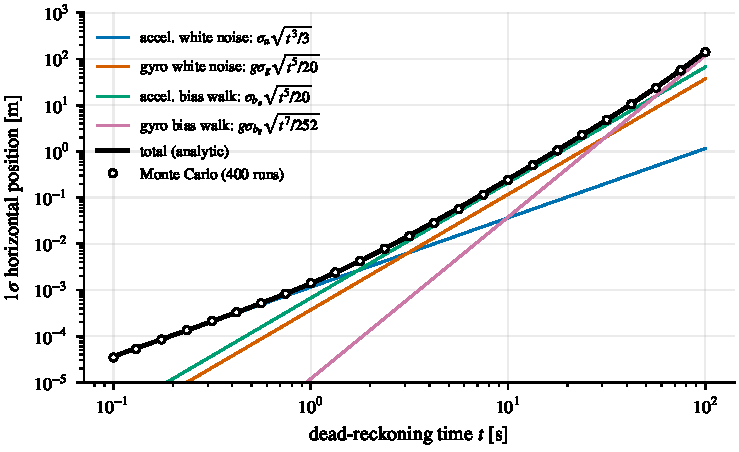
\includegraphics[width=0.88\textwidth]{fig_cov_growth.pdf}
  \caption{Horizontal position standard deviation of a dead-reckoning IMU with EuRoC noise parameters,
  from \eqref{eq:growth-laws}, with a Monte Carlo check (400 runs of the discretized error equations at
  200~Hz). Accelerometer white noise dominates for the first two seconds, the accelerometer bias walk from
  there to about a minute, and then the gyro bias walk takes over with its $t^{7/2}$ growth.}
  \label{fig:cov-growth}
\end{figure}

\begin{proposition}[Dead-reckoning growth laws]
\label{prop:growth-laws}
For a level, stationary IMU with zero initial uncertainty, the horizontal position variance grows as
\begin{equation}
  \sigma_p^2(t) = \underbrace{\frac{\sigma_a^2 t^3}{3}}_{\text{accel.\ white}}
  + \underbrace{\frac{g^2\sigma_g^2 t^5}{20}}_{\text{gyro white}}
  + \underbrace{\frac{\sigma_{b_a}^2 t^5}{20}}_{\text{accel.\ bias walk}}
  + \underbrace{\frac{g^2\sigma_{b_g}^2 t^7}{252}}_{\text{gyro bias walk}} .
  \label{eq:growth-laws}
\end{equation}
\end{proposition}
\begin{proof}
Accelerometer white noise is integrated twice ($m = 2$ in \cref{prop:integrated-noise}). Gyro white noise is integrated
once into tilt, scaled by $g$, and integrated twice more ($m = 3$). The accelerometer bias random walk is
itself integrated white noise, then integrated twice ($m = 3$). The gyro bias random walk adds one more
integration ($m = 4$). The sources are independent, so their variances add.
\end{proof}



\Cref{fig:cov-growth} evaluates \eqref{eq:growth-laws} with EuRoC's parameters. After one second of blind flight the
position uncertainty is about 1~mm, after ten seconds about 25~cm, and after a minute more than 10~m. The
camera's job is to keep the filter permanently in the left part of this plot.

\begin{projectlink}[Milestone 5]
The analytic check of M5 isolates the first term of \eqref{eq:growth-laws}: with $P_0 = 0$, only accelerometer noise and a
fixed orientation, the horizontal position variance must equal $\sigma_a^2t^3/3$. Because $\Phi$ and $Q_d$ are first-order
approximations, the agreement improves as $\Dt\to0$ (\cref{ex:double-integrator-qd}), and the test tolerance should reflect
that.
\end{projectlink}

\paragraph{Why diagonal entries need not grow monotonically.} The attitude covariance is expressed in body axes
(\cref{rem:cov-rotates}). When the vehicle rotates, the attitude block of $\Phi$ rotates the covariance between axes, so an
individual diagonal entry can shrink during pure propagation even though no information is gained. Monotonicity
holds for invariant quantities, such as the eigenvalues of $P_{\theta\theta}$ when the vehicle is not rotating, but not for
individual entries.

% ------------------------------------------------------------------------------
\section{Validating covariance propagation}

Two independent tests catch nearly all propagation bugs.

\paragraph{Finite differences on the discrete propagation.} The Jacobian of one step of the nominal integrator,
computed numerically with $\bplus/\bminus$, must match $\Phi$ column by column (the derivation exercise above). This
catches sign errors, transposes, and blocks placed at wrong indices. The test must use a non-trivial state.

\paragraph{Monte Carlo.} Simulate $M$ noisy IMU sequences from a known trajectory, integrate each with the nominal
equations from a perturbed initial state drawn from $P_0$, and compute the errors
$e^{(j)} = x_{\text{true}}\bminus\hat x^{(j)}$. Their sample covariance must agree with the propagated $P$. If the filter is
correct, the ratio of a sample variance to the predicted variance is distributed as $\chi^2_{M-1}/(M-1)$, so for
$M = 500$ it should lie in $[0.88, 1.13]$ with 95\% probability for each diagonal entry. Larger deviations, or many
entries near the bounds in the same direction, indicate an error in $G_c$, $Q_c$ or the units. This catches errors
that finite differences cannot, such as a wrong noise density or a missing $\Dt$.

\begin{takeaways}
\begin{itemize}
  \item The error state is 15-dimensional with the frozen layout $[\delta p, \delta v, \delta\theta, \delta b_a, \delta b_g]$.
  \item Error dynamics follow from substituting $x = \hat x\bplus\delta x$, subtracting the nominal dynamics, and keeping
        first-order terms. The perturbation convention changes the result.
  \item $\Phi \approx I + F_c\Dt$, $Q_d \approx G_cQ_cG_c\T\Dt$ with continuous densities; clones have identity dynamics.
  \item Position variance grows like $t^3$ (accel.\ noise), $t^5$ (gyro noise, accel.\ bias walk) and $t^7$ (gyro bias walk).
  \item Validate $\Phi$ by finite differences and $P$ by Monte Carlo with statistically justified bounds.
\end{itemize}
\end{takeaways}

\begin{exercises}
  \item Derive the velocity error dynamics for the global perturbation, and compare its structure with your local
        result. Which one depends on the vehicle's heading?
  \item Using your $F_c$, show that $\delta\theta$ is decoupled from $\delta p$ and $\delta v$, and explain this from the cascade structure.
  \item Starting from \eqref{eq:imu-discretization}, write $Q_d$ block by block and check its units.
  \item Implement covariance propagation for the 15-state system in Python and reproduce \cref{fig:cov-growth}, including
        the Monte Carlo points.
  \item For a vehicle rotating about its $z$-axis at 1~rad/s with $P_{\theta\theta} = \diag(10^{-4}, 10^{-6}, 10^{-6})$, propagate
        $P_{\theta\theta}$ for a quarter turn with no noise and observe the diagonal entries.
  \item How large must $M$ be for a Monte Carlo variance check to detect a 10\% error in $\sigma_a$ with high probability?
\end{exercises}
